%--------------------
% Packages
% -------------------
\documentclass[11pt]{article}



\usepackage[pdftex]{graphicx} % Required for including pictures
\usepackage[pdftex,linkcolor=black,pdfborder={0 0 0}]{hyperref} % Format links for pdf
\usepackage{calc} % To reset the counter in the document after title page
\usepackage{enumitem} % Includes lists

\frenchspacing % No double spacing between sentences
\linespread{1.2} % Set linespace
\usepackage[a4paper, lmargin=0.1666\paperwidth, rmargin=0.1666\paperwidth, tmargin=0.1111\paperheight, bmargin=0.1111\paperheight]{geometry} %margins
%\usepackage{parskip}

\usepackage[all]{nowidow} % Tries to remove widows
\usepackage[protrusion=true,expansion=true]{microtype} % Improves typography, load after fontpackage is selected

\usepackage{lipsum} % Used for inserting dummy 'Lorem ipsum' text into the template
\usepackage{amsfonts}
\usepackage{csquotes}

\newcommand{\XX}{$\mathbb{X}$ }
\newcommand{\OO}{$\mathbb{O}$ }

%-----------------------
% Set pdf information and add title, fill in the fields
%-----------------------
\hypersetup{ 	
pdfsubject = {},
pdftitle = {},
pdfauthor = {}
}

%-----------------------
% Begin document
%-----------------------
\begin{document} %All text i dokumentet hamnar mellan dessa taggar, allt ovanför är formatering av dokumentet

\section{Introduction}

Tic Tac Toe is a fun two-player game that can be played on pen and paper. A 3x3 grid is drawn on the page and the players alternate marking an empty square on the grid. The goal of the game is to get three of your marks in a straight line; that is, a horizonal, vertical, or diagonal line.

The original version of Tic Tac Toe is not usually played by adults, because it is very simple. If both players have optimal strategy, every game results in a draw, which makes the game futile.\footnote{https://mathworld.wolfram.com/Tic-Tac-Toe.html} Indeed, it is not hard for an adult to play a perfect game, since there aren't that many squares on the board and all possibilities can be considered.

Qubic is a variation of Tic Tac Toe that is in 3D. Traditionally, the size of the game board is 4x4x4 (for reasons that will be explained below), but in this report the 3x3x3 variant will be considered for simplicity's sake. This game has the same rules as Tic Tac Toe: players alternate placing their marks on empty cubes on the board. The goal of the game is to get a row of 3. However, now there are rows of 3 that are parallel to the x, y, and z axes, as well as diagonals in the xy, yz, and xz planes, and even diagonals spanning all three axes.

\begin{figure}[h]
    \centering
    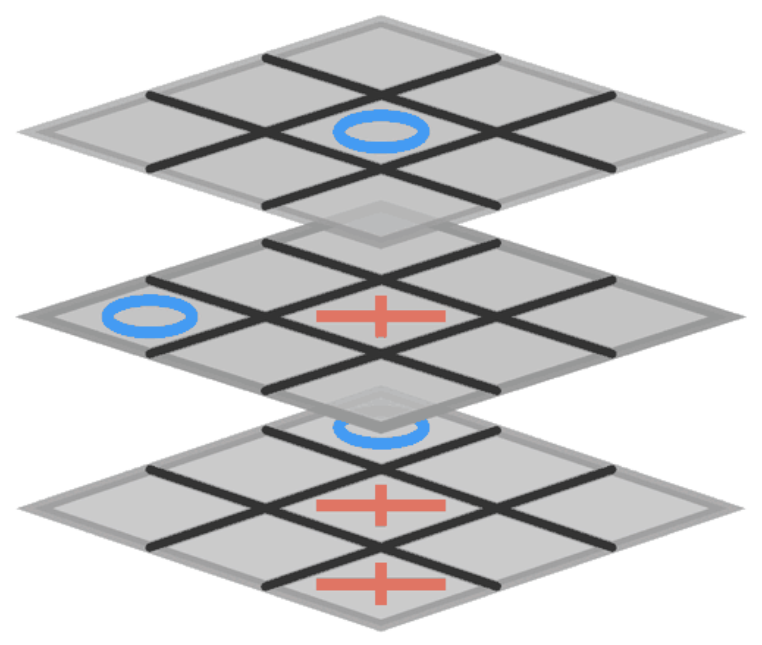
\includegraphics[width=0.5\textwidth]{qubic}
    \caption[An image of a Qubic board]{An image of a Qubic board\footnotemark}
    \label{fig:qubic}
\end{figure}

\footnotetext{Image from Chang math blog}

Technically speaking, 3x3x3 Qubic is also a futile game, since an optimal player who plays first is guaranteed to win every time.\footnote{4x4x4 Qubic also has a first-player-wins strategy, however it is much more complicated than the 3x3x3, which is why it is a more popular variant. \url{http://library.msri.org/books/Book42/files/golomb.pdf}} However, due to the complexity of visualizing the game in three dimensions and the number of possible rows, the average adult player has a much harder time considering all possibilities, resulting in games that are more evenly matched and interesting.

\subsection{Notation and terminology}
This report will include some mathematical notation and terminology, which will be defined in this section. 

The 3D gameboard is referred to as the "hyperboard". We will let $c_{x}$ represent the value of the cube at position $x$, where $x$ is a 3-tuple of integers in the range 0-2 inclusive. The cube positions will be indexed from 0; therefore, the top left back corner is (0, 0, 0) and the bottom right front corner is (2, 2, 2).

A triple is a row of three cubes that are in a vertical, horizontal, or diagonal line through the cube. If a player occupies all the cubes in a triple with their mark, then they have won. Mathematically, a set of three coordinates $\{x, y, z\}$ is a triple if and only if $y = v + x$ and $z = 2v + x$, where $v$ is one of \{$(1, 0, 0)$, $(0, 1, 0)$, $(0, 0, 1)$, $(1, 1, 0)$, $(1, 0, 1)$, $(0, 1, 1)$, $(1, 1, 1)$, $(1, 1, -1)$, $(1, -1, 1)$, $(1, -1, -1)$\}. Examples of triples include $\{(0, 0, 0), (0, 1, 0), (0, 2, 0)\}$ and $\{(0, 0, 0), (1, 1, 1), (2, 2, 2)\}$.

The marks on the board will be represented by \XX and \OO to differentate them from the letters X and O. Often, the marks are represented by integers rather than symbols in the models, and the convention used in this paper is that \XX and \OO are represented by 1 and -1, respectively.



\section{CSPs}
The Constraint Satisfaction Problem (herein referred to as CSP) is the problem of selecting values for one or more integer variables that satisfies some contraint. For example, if you have three variables, $x, y, z$ that are all in the range $0...3$, and you are trying to satisfy the constraint $3x + 2yz < 5$, the CSP solver would return solutions such as $(x,y,z) = $ (0, 0, 0), (1, 0, 0), (1, 1, 0), etc.

In this case, we need a way to model the game Qubic as a CSP.

\subsection{Model}
In the model, we will have a variable representing each of the cubes in Qubic. A value of zero for one of the variables will represent that the corresponding cube is empty; 1 represents an \XX; and -1 represents an \OO. The model will take as input the current state of the board, and will return a single move that should be taken next. In this case, the model will only ever play on behalf of \OO, and as such it will always optimize for \OO to win.

Individual CSP models are too simple to encode the logic for an advanced Qubic player: a CSP can only represent one strategy, but there are different strategies depending on the situation that you are in. The general strategy breaks down as follows:\footnote{These rules are loosely based off of the algorithm from Newell and Simon, \url{https://onlinelibrary.wiley.com/doi/epdf/10.1207/s15516709cog1704_3}}
\begin{enumerate}
    \item[(a)] If there is a winning move, you should take it.
    \item[(b)] If the opponent will have a winning move next turn, you should try to block it, if possible.
    \item[(c)] Otherwise, you should try to work towards making a triple for yourself.
\end{enumerate}
One sub-model will be designed for each strategy. The sub-models will be utilized in series: that is, the first sub-model will be run, and if a suitable solution is found, it will make that move. Otherwise, an attempt to find solution for the second sub-model will begin, and if it is successful it will take that move. Finally, if the first two sub-models fail, the last sub-model will select the move.

\subsubsection{Constraints common to all sub-models}
Regardless of which sub-model is being used, there are a few common constraints which apply. Firstly, any space which is currently occupied with an \XX or \OO must remain that way. In other words, the model may not opt to change the mark of a cube which has already been played. Secondly, the model may only play one new move per turn. For example, it can not add two new \OO's on its turn to make a win.

\subsubsection{Winning Sub-model}
The winning sub-model will attempt to find a way for the current player to get a row of three cubes. Mathematically, that means there exists a triple of coordinates $x, y, z$ such that
$$ c_x + c_y + c_z = -3.$$
In other words, there should be exactly one triple of cubes such that the the sum of the cubes is -3.

For technical reasons related to limitations of the solver, additional variables were needed. One boolean variable for each of the triples was created. A contraint was added that stipulates that exactly one of them should be true. Then, the constraint from the previous paragraph is only to be enforced if the boolean variable corresponding to that triple was true. This enforces the ``exactly one" constraint.

\subsubsection{Opponent win prevention sub-model}
The opponent win prevention sub-model will attempt to find a way to prevent the opponent from winning. In this model, the constraint will be that for every triple of coordinates $x, y,z$, $$c_x + c_y + c_y < 2.$$ That is, the sum of every triple of cubes will be less than 2.

This effectively prevents a win. The cases can be broken down by the number of X's in a row. If there are 0 or 1 \XX's in a row, there is not a threat of the opponent winning. If there are 2 \XX's to begin with, this constraint enforces that an \OO must be placed in the third square (otherwise, the sum of the triple of cubes would be 2, which is not permissible). This covers all cases, since in the case of 3 \XX's, the opponent has already won and this can not be prevented. 

This model will only work if there is exactly one triple in which the opponent is threatening a win. In the case where there are two or more threats where the opponent may win, the model may not be able to be satisfied because the model may only place one mark per turn. This edge case will be handled by the last submodel.

\subsubsection{Optimal "other" move}
The first two models have specific purposes: to win and to prevent the opponent from winning, respectively. However, there are a lot of situations where neither of those goals are attainable, and the models will not be satisfiable. This final model serves as a catch-all that plays a move in any circumstance.

Ideally, it would not just select a random move to play. Out of all the legal moves, it would optimize over a few metrics. Firstly, if there are multiple different ways for an opponent to win, it would take away one of those opportunities in the hope that the opponent will miss the other (in Qubic, it can be hard to visualize all possible moves, and a human opponent may miss one). If that isn't possible, then it would try to make a move which sets it up for a win.

Unfortunately, I was not able to get Google's ORTools library to optimize in this fashion. There is an optimization function that can be applied to the CSP, but it was poorly documented and I was not able to figure it out in time. My model just selects a random move.


\subsection{Results and discussion}
The CSP is ok at the game. 


\section{Planning}
The next AI technique that will be applied to Qubic is Automated Planning. In this technique, there will be a model which specifies the Fluents (variables which characterize the state), Actions ("moves" that can be made to transform from one state to the next), Initial State (set of fluents which are initially true), and Goal State (set of fluents that we want to be true in the end). The input of a planner is the initial state, and the output is a plan, which is a sequence of actions to be taken which take you from the initial state to the goal state.

The usual flavour of planning covers situations that are deterministic (after every action, you know exactly what the resulting state is) and fully observable (you know the whole state). However, this case is not deterministic, since the opponent is free to play whichever move they want in response to your move. Therefore, we must use a more advanced planner called the Fully Observable Non Deterministic Planner (FOND Planner).\footnote{\url{https://www.cs.toronto.edu/~sheila/publications/mui-mci-bel-icaps14.pdf}} In the case of FOND planners, the input is still the initial state, but the output becomes a ``policy", which is a list of if-then rules: if the state is this, then take that move.


\subsection{Model}
The model has the following constants:
\begin{itemize}
    \item \texttt{cellxyz}: represents the cell at $(x, y, z)$, where $(x, y, z)$ is a coordinate. For example, \texttt{cell012} is the cell at (0, 1, 2)
    \item \texttt{mark-x, mark-o}: represents an \XX and \OO, respectively
\end{itemize}

\noindent In my model, there are the following fluents:
\begin{itemize}
    \item \texttt{(cell-mark ?cell - cell ?mark - mark)}: This represents the mark that each cell holds; specifically, that cell \texttt{?cell} has mark \texttt{?mark}
    \item \texttt{(x-turn)} represents if it is currently \XX's turn
    \item \texttt{(won ?winner - mark)} represents the winner of the game. \XX wins if \texttt{(won mark-x)}, and \OO wins if \texttt{(won mark-o)} 
    \item \texttt{(check-required)} represents when a check is required to see if a player has won
    \item \texttt{(dead-end)} is used to prevent the planner from playing twice on a certain cube
\end{itemize}

\noindent There are the following actions:
\begin{itemize}
    \item \texttt{(play-x ?cell)}: plays an \XX on the board in the \texttt{?cell}. The preconditions are that \texttt{?cell} is empty, it's \XX's turn, no check is required, and neither player has won yet. The effect is that \texttt{?cell} is marked with an \XX, it's no longer \XX's turn, and a check is required.
    \item \texttt{(play-o)}: plays an \OO on the board. The preconditions are that \texttt{?cell} is empty, it's not \XX's turn, a check isn't required, and no player has won yet. The effect is non-deterministic: the opponent is allowed to mark \OO at any location that is not currently occupied. Regardless of the opponent's move, a check is required and it becomes \XX's turn.
    \item \texttt{(check)}: checks the board to see if either player has won. The precondition is that a check is required. The effect is that check is no longer required, and if either player has won, it will set the \texttt{won} fluent for that player.
\end{itemize}

\noindent The \texttt{(play-x ?cell)} action is straightfoward. However, the \texttt{(play-o)} and \texttt{(check)} actions require some discussion. The former works by using the \texttt{oneof} keyword that is part of FOND planning, which specifies the possible effects of a non-deterministic action. Each of the possible effects corresponds to the player playing one of the cubes. I will show the PDDL of one of the possible effects then explain it below:\\
\texttt{(and \\
    \indent (when \\
    \indent \indent (cell-mark ?cell mark-empty) \\
    \indent \indent (and (not (cell-mark ?cell mark-empty)) (cell-mark ?cell mark-o))\\
    \indent )\\
    \indent (when \\
    \indent \indent (not(cell-mark ?cell mark-empty)) \\
    \indent \indent (dead-end) \\
    \indent)\\
)}

This PDDL works by handling two conditions using conditional effects. If the cell that is selected is empty, the effect is that the cell will be marked with an \OO (making it not empty anymore). Otherwise, the cell selected by the opponent is not empty (i.e. it has a mark), in which case the effect is \texttt{dead-end}. There is no way to get out of a dead end, and the goal explicitly says that there must not be a dead end in the plan, so this prevents the planner from exploring plans where the opponent marks on top of a cell that has already been marked.

The latter action works by using a bunch of conditional effects. Each of the winning triples is encoded, and if any of them are marked with the same mark, then it will result in a win for the mark that occupies that triple. This marks the end of the plan, either successfully or unsuccessfully depending on which mark occupied the triple.

In general, the order of actions is: \texttt{play-x, check, play-o, check, play-x..., check}, until either \XX or \OO wins.

\subsection{Results and discussion}
To verify that the model actually works and generates a suitable plan, I first removed the non-deterministic aspect of the model and allowed the planner to play on behalf of both players. This is the plan that it came up with:
\begin{displayquote}
\texttt{(play-x cell000)\\
(check )\\
(play-o cell222)\\
(check )\\
(play-x cell001)\\
(check )\\
(play-o cell221)\\
(check )\\
(play-x cell002)\\
(check )}
\end{displayquote}

This plan accomplishes the goal (\XX wins the game), so it appears that the model correctly represents the setting.

During the process of modelling this setting, I found that not all models were built equal. My initial naive model was extremely inefficient. I used to check if the game had been won in the Goal section of the PDDL. When I went to generate the plan, after 30 minutes it had used up 57GB of RAM and still hadn't solved the problem yet. I put the win checking logic as an effect of the playing actions, but then it wouldn't register a win until a round later than the win was accomplished. Finally, using a \texttt{(check)} action to check if there is a winner solved both issues.

Moving from the deterministic to non-deterministic model was also challenging. Quantifiers are not supported yet for non-deterministic effects, so I couldn't say ``the effect is that one of the empty cells is marked with an \OO". This problem was solved by using the \texttt{dead-end} fluent. Another challenge with non-deterministic planning was verifying that the policy was correct. Ideally, I would have implemented a program that visualized it with a nice custom graph, but I did not have time.

To verify the policy, I went through the policy.out file, painstakingly verifying a few states to ensure that suitable moves were performed to cause a win and prevent the opponent from winning. I also examined the graph output by the \texttt{prpviz} utility. It is too large to include in its entirety in this report, so I included a cropped version below -- the whole version can be found on the GitHub repo for this project.

\begin{figure}[h]
    \centering
    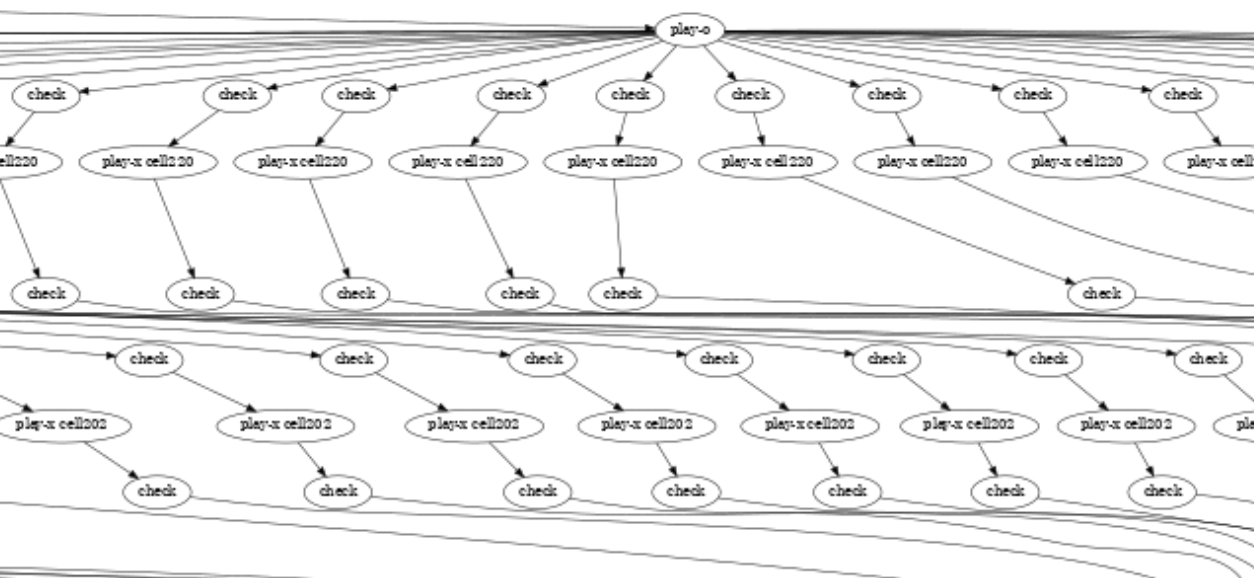
\includegraphics[width=0.75\textwidth]{policyviz}
    \caption{A very small snippet of the policy visualization}
    \label{fig:policyviz}
\end{figure}

\section{Deep Neural Network}
The final approach that will be applied to Qubic is a Deep Neural Network. A deep neural network is a neural network that has multiple hidden layers. These networks are powerful because they don't require the user to manually come up with the input features: the features are learned as part of the training process.

One of the biggest limitations of deep neural networks is that they require a large amount of training data to be effective. Thankfully, Qubic is an ideal setting because there are a large amount of board states, and it is easy to generate training data on the fly. 

I will first show how I generated the training data. Next, I will discuss what the model's inputs and outputs represent. Then, I will explain the two models under consideration: Model 1 will follow a traditional deep neural network approach; Model 2 will exploit the fact that there is a lot of symmetry in the game Qubic to see if we can obtain similar accuracy with a lot fewer weights.

\subsection{Training data}
As previously mentioned, it is trivial to generate training data. Functionality was added to the Qubic class to generate a random game. The random games were generated as follows:
\begin{enumerate}
    \item A blank game was initialized
    \item Out of all the cells that are empty, a random one was chosen. The current player's mark was placed there
    \item Step 2 was repeated until there is a winner
\end{enumerate}
Each intermediary hyperboard was associated with the eventual result of the game, forming a tuple that was used as training data.

Suppose that 1,000 training points needed to be generated. A new random game would be generated, and suppose that it was 9 moves long. Then, all 9 of those (hyperboard, winner) pairs would be used as training data. The process will repeat for the remaining 993 training pairs, until all the required data is generated.

250,000 data points were used to train model 1, and 2,500 were used to train model 2.

\subsection{Model input / outputs}
The model will accept a hyperboard as input, and return a tuple $(x, y)$, where $x$ and $y$ represent the model's prediction of the probability that \XX and \OO will win, respectively. This can be used to determine which move should be taken next: if the model is playing on behalf of \XX, it should take the move that has the highest probability of \XX winning. 

\subsection{Model 1}
The first model that is being examined is a traditional, densely connected deep neural network. The architecture is as follows:\footnote{Inspiration for these hyperparameters comes from the following article: \url{https://medium.com/swlh/tic-tac-toe-and-deep-neural-networks-ea600bc53f51}}
\begin{itemize}
    \item Dense layer, 200 outputs, ReLu activation
    \item Dropout layer with parameter of 0.2
    \item Dense layer, 125 outputs, ReLu activation
    \item Dense layer, 75 outputs, ReLu activation
    \item Dropout layer with parameter of 0.1
    \item Dense layer, 25 outputs, ReLu activation
    \item Dense layer, 2 outputs, Softmax activation
\end{itemize}

The model was trained with a categorical cross-entropy loss function  and its output activation function is a softmax, since it is a multi-class classifier.

\subsection{Model 2}
The astute reader may have noticed that Qubic has a lot of symmetry. Practically speaking, Qubic is just a bunch of Tic Tac Toe games that share some cells and are being played out simultaneously. Model 2 will attempt to exploit that symmetry to reduce the size of the model without impacting performance.

The model works by dividing the hyperboard into ``slices", each of which  corresponds to a Tic Tac Toe board; that is, the slices in the xy, xz, and yz planes as well as the diagonal slices. It will use a deep neural network trained on Tic Tac Toe to generate the probabilities of each slice winning, losing, or drawing. Then, those probabilities will be aggregated into a new vector, which will be fed to a smaller neural network that will attempt to predict the winner of the game. Conceivably, this would result in a model that is smaller: the redundancy of learning Tic Tac Toe in 3D would be eliminated, and would be replaced by the much simpler tasks of learning Tic Tac Toe in 2D and combining the slices' probabilities together.

I did not write the code to generate the 2D Tic Tac Toe model. I took it from \url{https://medium.com/swlh/tic-tac-toe-and-deep-neural-networks-ea600bc53f51}. I wrote the code that converts hyperboards to slices, and the code of the model that combines the probabilities. Its architecture is:
\begin{itemize}
    \item Dense layer, 50 neurons, ReLu activation
    \item Dense layer, 25 neurons, ReLu activation
    \item Dense layer, 2 outputs, Softmax activation
\end{itemize}

It was trained with a categorical cross-entropy loss function and softmax output activation function, for the same reasons as model 1.

\subsection{Results and discussion}
To establish a baseline, we begin by assuming that the players' moves are totally random. Out of 1000 simulations that were run, \XX won 558 and \OO won 442 times. Using the Two-Proportions Z test, we note that \XX has a statistically significant advantage ($p = 0.01$) as the first player to go.

The simulation was run with model 1 representing \XX and \OO using a random strategy, and in these 1000 simulations \XX won 896, giving it a significant improvement over baseline. When the roles were reversed and model 1 represented \OO, it won 803 times, also much better than baseline. Both of these results are statistically significant ($p < 0.001$), which means that the model is better than random at playing Qubic.

Theoretically, as the first player, \XX can win every time. Model 1's 90\% win rate is impressive, but it would be an interesting exercise to try to increase the win rate, potentially to 100\%. There are $3^{27}$ possible board states, which is much higher than the number of data points that the model was trained on, so it may benefit from more training.

Model 2 took so long to run that it was practically infeasible to run 1000 simulations. 10 simulations were run with model 2 representing \XX and \OO random, and \XX won 6 out of 10 times. This is not a statistically significant improvement over baseline.

The reason that model 2 takes so long is that it has to do a lot more inferences. For every candidate move (there could be up to 27), it has to use the Tic Tac Toe model on each of the slices (there are 11), and then perform an inference on all of the results from the slices. There multiple moves per game, and therefore there are often multiple thousand inferences per game. Any potential space savings from using the two models like this are outweighed by the large time increase to do the inference.

It is unclear why model 2 performs so poorly. Due to the large amount of time required to do inference, the size of the training data had to be much smaller, which could have contributed to the bad performance. Additionally, the network may not have been deep or wide enough. There are too many variables to be able to narrow down the source of the bad performance.

\section{Conclusion}
In this report, three AI techniques were applied to the game Qubic. 

First was CSPs. CSPs were a promising technique.

Then, Automated Planning was applied.

\end{document}